%%%%%%%%%%%%%%%%%%%%%%%%%%%%%%%%%%%%%%%%%
% Masters/Doctoral Thesis
% LaTeX Template
% Version 1.41 (9/9/13)
%
% This template has been downloaded from:
% http://www.latextemplates.com
%
% Original authors:
% Steven Gunn
% http://users.ecs.soton.ac.uk/srg/softwaretools/document/templates/
% and
% Sunil Patel
% http://www.sunilpatel.co.uk/thesis-template/
%
% License:
% CC BY-NC-SA 3.0 (http://creativecommons.org/licenses/by-nc-sa/3.0/)
%
% Note:
% Make sure to edit document variables in the Thesis.cls file
%
%%%%%%%%%%%%%%%%%%%%%%%%%%%%%%%%%%%%%%%%%

%----------------------------------------------------------------------------------------
%	PACKAGES AND OTHER DOCUMENT CONFIGURATIONS
%----------------------------------------------------------------------------------------

%\documentclass[11pt, twoside]{Thesis} % Paper size, default font size and two-sided paper

\documentclass[10 pt, a4paper, twoside, openright]{Thesis}
%\special{papersize=297mm,210mm}% it is A4 paper size, I got from Wikipedia.
\special{papersize=240mm,170mm}% it is the weird format of MPI thesis
\usepackage{blindtext}
\usepackage[T1]{fontenc}
\usepackage{lmodern}
\usepackage{textcomp}
\usepackage{tabularx}
\usepackage{tabu}
\usepackage{pdfx}
\usepackage{booktabs}
\usepackage{setspace}
\usepackage{multirow}
\usepackage{array}
\usepackage{afterpage}
\usepackage{longtable}
\usepackage{lscape}
%\usepackage{cite}
\usepackage{chngcntr}
\usepackage{url}
\urlstyle{same}
%\usepackage{fontspec}
%\newcommand{\TextUnderscore}{\rule{.2em}{.1pt}}
\DeclareGraphicsRule{.ai}{pdf}{.ai}{}
\DeclareGraphicsExtensions{.pdf,.png,.jpg,.ai,.eps}
\graphicspath{{Figures/}}
\usepackage[dvipsnames]{xcolor}
%\usepackage[sectionbib]{chapterbib}
\usepackage{textgreek}
\usepackage{float}
\usepackage{chemformula}
\usepackage{textcomp}
\usepackage{acronym}
\usepackage{wasysym}
\usepackage[english]{babel}
\usepackage[comma, sort&compress]{natbib} % Use the natbib reference package - read up on this to edit the reference style; if you want text (e.g. Smith et al., 2012) for the in-text references (instead of numbers), remove 'numbers'
\usepackage{caption}
\usepackage{pdfpages}
\usepackage{gensymb}
%\DeclareCaptionLabelFormat{myformat}{#1 #2}
%\captionsetup{within=none,labelformat=myformat}
\hypersetup{urlcolor=black, colorlinks=true} % Colors hyperlinks in blue - change to black if annoying
\title{\ttitle} % Defines the thesis title - don't touch this
%\usepackage[hmarginratio=2:3]{geometry}
\usepackage[titletoc]{appendix}

\newcommand{\beginsupplement}{%
        \setcounter{table}{0}
        \renewcommand{\thetable}{S\arabic{chapter}.\arabic{table}}%
        \setcounter{figure}{0}
        \renewcommand{\thefigure}{S\arabic{chapter}.\arabic{figure}}%
     }
\newcommand{\nosupplement}{%
        \setcounter{table}{0}
        \renewcommand{\thetable}{\arabic{chapter}.\arabic{table}}%
        \setcounter{figure}{0}
        \renewcommand{\thefigure}{\arabic{chapter}.\arabic{figure}}%
        }

\begin{document}

\selectlanguage{english}
\sloppy
\frontmatter % Use roman page numbering style (i, ii, iii, iv...) for the pre-content pages

\setstretch{1.3} % Line spacing of 1.3

%try default
%\fancyhead[LE,RO]{\slshape \rightmark}
%\fancyhead[LO,RE]{\slshape \leftmark}
%\fancyfoot[C]{\thepage}
%\headrulewidth 0.4pt
%\footrulewidth 0 pt



% Define the page headers using the FancyHdr package and set up for one-sided printing
%\fancyhead{} % Clears all page headers and footers
%\usepackage{fancyhdr}
%\pagestyle{fancy}
%\fancyhead[RO,LE]{\thepage}
%\fancyhead[LE,RO]{\thepage}
%\rhead{\thepage} % Sets the right side header to show the page number
%\lhead{} % Clears the left side page header

%\pagestyle{fancy} % Finally, use the "fancy" page style to implement the FancyHdr headers

\newcommand{\HRule}{\rule{\linewidth}{0.5mm}} % New command to make the lines in the title page

% PDF meta-data
%\hypersetup{pdftitle={\ttitle}}
%\hypersetup{pdfsubject=\subjectname}
%\hypersetup{pdfauthor=\authornames}
%\hypersetup{pdfkeywords=\keywordnames}

%----------------------------------------------------------------------------------------
%	TITLE PAGE
%----------------------------------------------------------------------------------------

\begin{titlepage}

\begin{center}


%\vspace{2cm}

%\large Dissertation
\vspace*{2cm}

{\huge \textbf{\ttitle}\par}
\thispagestyle{empty}
\vspace{1.5cm}
Dissertation \\
zur Erlangung des Doktorgrades \\
der Naturwissenschaften \\
- Dr.\ rer.\ nat. - \\ % University requirement text
\vspace{1cm}
dem Fachbereich Biologie/Chemie \\
der Universit\"{a}t Bremen \\
vorgelegt von

\vspace{1.5cm}

\textbf{My name}
\null{}
\vfill
{\large{Bremen, Mai 2018}}\\[4cm] % Date
\cleardoublepage{}
\vspace*{2cm}

{\huge \textbf{\ttitle}\par}
\thispagestyle{empty}

\vspace{1.5cm}
A thesis submitted to University of Bremen in \\
partial fulfillment for the degree of \\
DOCTOR OF SCIENCE (Doktor der Naturwissenshaften) \\
\vspace{1.5cm}
University of Bremen\\
Faculty of Biology/Chemistry \\
\vspace{1.5cm}

\textbf{My name}
\vspace{2cm}
\vfill
{\large{Bremen, May 2018}}\\[4cm] % Date

%\textsc{\LARGE \univname}\\[1.5cm] % University name
%\textsc{\Large Doctoral Thesis}\\[0.5cm] % Thesis type


%\HRule % Horizontal line

%{\huge \textbf{\ttitle}\par}% Thesis title

%\HRule % Horizontal line

%\begin{minipage}{0.4\textwidth}
%\begin{flushleft} \large
%\emph{Author:}\\

%\end{flushleft}
%\end{minipage}
%\begin{minipage}{0.4\textwidth}
%\begin{flushright} \large
%\emph{Supervisor:} \\

%\end{flushright}
%\end{minipage}\\[3cm]

%\vspace{2cm}

%\large Dissertation

%~\\zur Erlangung des Doktorgrades
%~\\der Naturwissenschaften
%~\\- Dr. rer. nat. - \\[0.3cm] % University requirement text
%\vspace{3cm}
%dem Fachbereich Biologie/Chemie
%~\\der Universit\"at Bremen
%~\\vorgelegt von

%\vspace{2.5cm}

%\vfill
\end{center}

\end{titlepage}

\newpage
\pagestyle{empty}


\begin{minipage}{0.3\textwidth}
\end{minipage} \hfill
\begin{minipage}{0.7\textwidth}
Die vorliegende Doktorarbeit wurde im Rahmen des Programms International \textit{Max Planck Research School of Marine Microbiology} (MarMic) in der Zeit von Januar 2015 bis Juni 2018 am Max-Planck-Institut f\"ur Marine Mikrobiologie angerfertigt. \\

This thesis was prepared  under the framework of the International Max Planck Research School of Marine Microbiology (MarMic) at the Max Planck Institute for Marine Microbiology from January 2015 to June 2018.\\
\end{minipage}


\null{}
\vfill{}
~\\Gutachter: Prof.\ Dr.\ John Doe
~\\Gutachter: Prof.\ Dr.\ John Doe
~\\
~\\Pr\"ufer: Prof.\ Dr.\ John Doe
~\\Pr\"ufer: Dr.\ John Doe


%----------------------------------------------------------------------------------------
%	DECLARATION PAGE
%	Your institution may give you a different text to place here
%----------------------------------------------------------------------------------------

%\Declaration{

%\addtocontents{toc}{\vspace{1em}} % Add a gap in the Contents, for aesthetics

%I, \authornames, declare that this thesis titled, '\ttitle' and the work presented in it are my own. I confirm that:

%\begin{itemize}
%\item[\tiny{$\blacksquare$}] This work was done wholly or mainly while in candidature for a research degree at this University.
%\item[\tiny{$\blacksquare$}] Where any part of this thesis has previously been submitted for a degree or any other qualification at this University or any other institution, this has been clearly stated.
%\item[\tiny{$\blacksquare$}] Where I have consulted the published work of others, this is always clearly attributed.
%\item[\tiny{$\blacksquare$}] Where I have quoted from the work of others, the source is always given. With the exception of such quotations, this thesis is entirely my own work.
%%\item[\tiny{$\blacksquare$}] I have acknowledged all main sources of help.
%\item[\tiny{$\blacksquare$}] Where the thesis is based on work done by myself jointly with others, I have made clear exactly what was done by others and what I have contributed myself.\\
%\end{itemize}

%Signed:\\
%\rule[1em]{25em}{0.5pt} % This prints a line for the signature

%Date:\\
%\rule[1em]{25em}{0.5pt} % This prints a line to write the date
%}

\clearpage % Start a new page

%----------------------------------------------------------------------------------------
%	QUOTATION PAGE
%----------------------------------------------------------------------------------------

\pagestyle{empty} % No headers or footers for the following pages

\null\vfill\vfill\vfill\vfill % Add some space to move the quote down the page a bit


\begin{flushright}
Dedication goes here
\end{flushright}

\vfill\vfill\vfill\vfill\vfill\vfill\null{} % Add some space at the bottom to position the quote just right

\clearpage % Start a new page

\pagestyle{empty} % No headers or footers for the following pages

\null\vfill % Add some space to move the quote down the page a bit

\vfill\vfill\vfill\vfill\vfill\vfill\null{} % Add some space at the bottom to position the quote just right

%\clearpage % Start a new page
\cleardoublepage{}

%----------------------------------------------------------------------------------------
%	ABSTRACT PAGE
%----------------------------------------------------------------------------------------

%\addtotoc{Summary} % Add the "Abstract" page entry to the Contents

%\abstract{\addtocontents{toc}{\vspace{1em}} % Add a gap in the Contents, for aesthetics



\clearpage % Start a new page

%----------------------------------------------------------------------------------------
%	ACKNOWLEDGEMENTS
%----------------------------------------------------------------------------------------

%\setstretch{1.3} % Reset the line-spacing to 1.3 for body text (if it has changed)

%\acknowledgements{\addtocontents{toc}{\vspace{1em}} % Add a gap in the Contents, for aesthetics

%The acknowledgements and the people to thank go here, don't forget to include your project advisor\ldots
%}
%\clearpage % Start a new page

%----------------------------------------------------------------------------------------
%	LIST OF CONTENTS/FIGURES/TABLES PAGES
%----------------------------------------------------------------------------------------

\pagestyle{fancy} % The page style headers have been "empty" all this time, now use the "fancy" headers as defined before to bring them back
\newpage
\chapter{Summary}
\chaptermark{}
\renewcommand{\chaptermark}[1]{\markboth{#1}{}}
\renewcommand{\sectionmark}[1]{\markright{#1}}
\fancyhead[RE]{\small}
% Section in the left on even pages}
\fancyhead[LO]{\small\rightmark}%Section in the left on odd pages

An english summary goes here

\newpage
\chapter{Zusammenfassung}
\chaptermark{}
\renewcommand{\chaptermark}[1]{\markboth{#1}{}}
\renewcommand{\sectionmark}[1]{\markright{#1}}
\fancyhead[RE]{\small}
% Section in the left on even pages}
%Section in the left on odd pages
\fancyhead[LO]{\small\rightmark}

A german summary goes here

\newpage
\clearpage % Start a new page
\section*{Abbreviations}
\setstretch{1} % Set the line spacing to 1.5, this makes the following tables easier to read

%\lhead{\emph{Abbreviations}} % Set the left side page header to "Abbreviations"

\begin{acronym}
\acro{ABC}{ATP-binding cassette}
\acro{ANI}{average nucleotide identity}
\end{acronym}



%\lhead{\emph{Table of Contents}} % Set the left side page header to "Contents"
\tableofcontents % Write out the Table of Contents

%\lhead{\emph{List of Figures}} % Set the left side page header to "List of Figures"
%\listoffigures % Write out the List of Figures

%\lhead{\emph{List of Tables}} % Set the left side page header to "List of Tables"
%\listoftables % Write out the List of Tables

%----------------------------------------------------------------------------------------
%	ABBREVIATIONS
%----------------------------------------------------------------------------------------



%\textbf{Acronym} & \textbf{W}hat (it) \textbf{S}tands \textbf{F}or \\


%----------------------------------------------------------------------------------------
%	PHYSICAL CONSTANTS/OTHER DEFINITIONS
%----------------------------------------------------------------------------------------

%\clearpage % Start a new page

%\lhead{\emph{Physical Constants}} % Set the left side page header to "Physical Constants"

%\listofconstants{lrcl} % Include a list of Physical Constants (a four column table)
%{
%Speed of Light & $c$ & $=$ & $2.997\ 924\ 58\times10^{8}\ \mbox{ms}^{-\mbox{s}}$ (exact)\\
% Constant Name & Symbol & = & Constant Value (with units) \\
%}

%----------------------------------------------------------------------------------------
%	SYMBOLS
%----------------------------------------------------------------------------------------

%\clearpage % Start a new page

%\lhead{\emph{Symbols}} % Set the left side page header to "Symbols"

%\listofnomenclature{lll} % Include a list of Symbols (a three column table)
%{
%$a$ & distance & m \\
%$P$ & power & W (Js$^{-1}$) \\
% Symbol & Name & Unit \\

%& & \\ % Gap to separate the Roman symbols from the Greek

%$\omega$ & angular frequency & rads$^{-1}$ \\
% Symbol & Name & Unit \\
%}

%----------------------------------------------------------------------------------------
%	DEDICATION
%----------------------------------------------------------------------------------------

\setstretch{1.3} % Return the line spacing back to 1.3

\pagestyle{empty} % Page style needs to be empty for this page

%\dedicatory{\ldots} % Dedication text

%\addtocontents{toc}{\vspace{2em}} % Add a gap in the Contents, for aesthetics

%----------------------------------------------------------------------------------------
%	THESIS CONTENT - CHAPTERS
%----------------------------------------------------------------------------------------

\mainmatter{}% Begin numeric (1,2,3...) page numbering

\pagestyle{fancy} % Return the page headers back to the "fancy" style

% Include the chapters of the thesis as separate files from the Chapters folder
% Uncomment the lines as you write the chapters
% Chapter 1

% Chapter Template

\chapter{Introduction} % Main chapter title

\label{Chapter1} % Change X to a consecutive number; for referencing this chapter elsewhere, use \ref{ChapterX}

%\lhead{Chapter 1. \emph{Introduction}} % Change X to a consecutive number; this is for the header on each page - perhaps a shortened title

\renewcommand{\chaptermark}[1]{\markboth{#1}{}}
\renewcommand{\sectionmark}[1]{\markright{#1}}
\fancyhead[RE]{\small\leftmark}
% Section in the left on even pages}
\fancyhead[LO]{\small\rightmark}%Section in the left on odd pages

\section{A section goes here}

I cite something~\citet{Fuhrman2015-dynamics}
\\
A figure

\begin{figure}[h!]
	\centering
	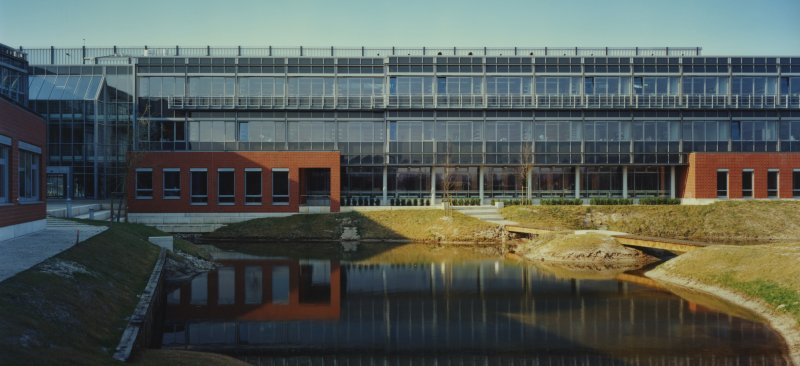
\includegraphics[width=0.6\textwidth] {Chap1_Fig1}
	\caption{\textbf{A figure example.} MMPI-MM.}\label{fig:C1Fig1}
\end{figure}

\blindmathpaper{2}

%\input{Chapters/Chapter5}
%\input{Chapters/Chapter6}
%\input{Chapters/Chapter7}

%%% acknoledgegements

%\input{{\acknowledgements{\addtocontents}} % Add a gap in the Contents, for aesthetics

%The acknowledgements and the people to thank go here, don't forget to include your project advisor\ldots
%}
%\addtocontents{toc}{\vspace{2em}} % Add a gap in the Contents, for aesthetics
%\acknowledgements % Cue to tell LaTeX that the following 'chapters' are Appendices
\let\cleardoublepage\clearpage
\addtocontents{toc}{\vspace{2em}} % Add a gap in the Contents, for aesthetics
\appendix % Cue to tell LaTeX that the following 'chapters' are Appendices
\begin{appendices}
\renewcommand\chaptername{Appendix}
\renewcommand{\chaptermark}[1]{\markboth{#1}{}}
\renewcommand{\sectionmark}[1]{\markright{#1}}
\fancyhead[RE]{\small\leftmark}
% Section in the left on even pages}
\fancyhead[LO]{\small\rightmark}%Section in the left on odd pages

\chapter[An appendix title]{An appendix title}% Main chapter title
\chaptermark{An appendix running title}

\label{Appendix1} % Change X to a consecutive number; for referencing this chapter elsewhere, use \ref{ChapterX}


\blindtext[10]

\end{appendices}

% Include the appendices of the thesis as separate files from the Appendices folder
% Uncomment the lines as you write the Appendices
%\chapter*{Bibliography}
\addcontentsline{toc}{chapter}{Bibliography}

%\chapter{Discussion and Perspectives} % Main chapter title

%\label{Chapter6} % Change X to a consecutive number; for referencing this chapter elsewhere, use \ref{ChapterX}

%\lhead{Chapter 6. \emph{Discussion and Conclusions}} % Change X to a consecutive number; this is for the header on each page - perhaps a shortened title


Adam P, Schneckenburger P, Schaeffer P, Albrecht P. (2000). Clues to early diagenetic sulfurization processes from mild chemical cleavage of labile sulfur-rich geomacromolecules. Geochim Cosmochim Acta 64:3485-3503.

Aller RC. (1994). Bioturbation and remineralization of sedimentary organic matter: effects of redox oscillation. Chem Geol 114:331-345.

Archer D, Maier-Reimer E. (1994). Effect of deep-sea sedimentary calcite preservation on atmospheric CO$_2$ concentration. Nature 367:260-263.

Armstrong RA, Lee C, Hedges JI, Honjo S, Wakeham SG. (2001). A new, mechanistic model for organic carbon fluxes in the ocean based on the quantitative association of POC with ballast minerals. Deep Sea Res Part II Top Stud Oceanogr 49:219-236.

Arndt S, J{\o}rgensen BB, LaRowe DE, Middelburg JJ, Pancost RD, Regnier P. (2013). Quantifying the degradation of organic matter in marine sediments: A review and synthesis. Earth-Science Rev 123:53-86.

Arnosti C. (2011). Microbial Extracellular Enzymes and the Marine Carbon Cycle. Ann Rev Mar Sci 3:401-425.

Arnosti C, Bell C, Moorhead DL, Sinsabaugh RL, Steen a. D, Stromberger M, et al. (2013). Extracellular enzymes in terrestrial, freshwater, and marine environments: perspectives on system variability and common research needs. Biogeochemistry 117:5-21.

Arrieta JM, Mayol E, Hansman RL, Herndl GJ, Dittmar T, Duarte CM. (2015). Dilution limits dissolved organic carbon utilization in the deep ocean. Science (80) 348:331-333.

Arthur MA, Dean WE, Pratt LM. (1988). Geochemical and climatic effects of increased marine organic carbon burial at the Cenomanian/Turonian boundary. Nature 335:714-717.

Badertscher S, Fleitmann D, Cheng H, Edwards RL, G\"okt\"urk OM, Zumb\"uhl a., et al. (2011). Pleistocene water intrusions from the Mediterranean and Caspian seas into the Black Sea. Nat Geosci 4:236-239.

Baird D, Christian RR, Peterson CH, Johnson GA. (2004). Consequences of hypoxia on estuarine ecosystem function: energy diversion from consumers to microbes. Ecol Appl 14:805-822.

Baird D, Ulanowicz RE. (1989). The seasonal dynamics of the Chesapeake Bay ecosystem. Ecol Monogr 59.

Ball DF. (1964). Loss-on-ignition as an estimate of organic matter and organic carbon in non-calcareous soils. J Soil Sci 15:84-92.

Baturin GN. (2007). Issue of the relationship between primary productivity of organic carbon in ocean and phosphate accumulation (Holocene-Late Jurassic). Lithol Miner Resour 42:318-348.

Belmar L, Molina V, Ulloa O. (2011). Abundance and phylogenetic identity of archaeoplankton in the permanent oxygen minimum zone of the eastern tropical South Pacific. FEMS Microbiol Ecol 78:314-26.

Bentley DR, Balasubramanian S, Swerdlow HP, Smith GP, Milton J, Brown CG, et al. (2008). Accurate whole human genome sequencing using reversible terminator chemistry. Nature 456:53-9.

Berelson WM, Hammond DE, McManus J, Kilgore TE. (1994). Dissolution kinetics of calcium carbonate in equatorial Pacific sediments. Global Biogeochem Cycles 8:219-235.

Bernardet J, Nakagawa Y, Holmes B. (2002). Proposed minimal standards for describing new taxa of the family Flavobacteriaceae and emended description of the family. Int J Syst Evol Microbiol 52:1049-1070.

Berner RA. (1990). Atmospheric carbon dioxide levels over phanerozoic time. Science 249:1382-6.

Berner RA. (1989). Biogeochemical cycles of carbon and sulfur and their effect on atmospheric oxygen over phanerozoic time. Palaeogeogr Palaeoclimatol Palaeoecol 75:97-122.

Berner RA. (1980). Early Diagenesis: A Theoretical Approach. First edit. Princeton University Press: Princeton, N.J.

Berner RA. (1969). Migration of iron and sulfur within anaerobic sediments during early diagenesis. Am J Sci 267:19-42.

Berner RA, Canfield DE. (1989). A new model for atmospheric oxygen over Phanerozoic time. Am J Sci 289:333-61.

B\"oer SI. (2008). Investigation of the distribution and activity of the benthic microorganisms in coastal habitats. University of Bremen.

B\"oer SI, Hedtkamp SIC, van Beusekom JEE, Fuhrman J a, Boetius A, Ramette A. (2009). Time- and sediment depth-related variations in bacterial diversity and community structure in subtidal sands. ISME J 3:780-91.

Boetius A, Albrecht S, Bakker K, Bienhold C, Felden J, Fernández-Méndez M, et al. (2013). Export of algal biomass from the melting Arctic sea ice. Science 339:1430-2.

Bopp L, Resplandy L, Orr JC, Doney SC, Dunne JP, Gehlen M, et al. (2013). Multiple stressors of ocean ecosystems in the 21st century: projections with CMIP5 models. Biogeosciences 10:6225-6245.

Br\"uchert V, J{\o}rgensen BB, Neumann K, Riechmann D, Schl\"osser M, Schulz H. (2003). Regulation of bacterial sulfate reduction and hydrogen sulfide fluxes in the central namibian coastal upwelling zone. Geochim Cosmochim Acta 67:4505-4518.

Brunet M-F, Cloetingh S. (2003). Integrated Peri-Tethyan Basins studies (Peri-Tethys Programme). Sediment Geol 156:1-10.

Çağatay MN, G\" or\" ur N, Flecker R, Sakınç M, T\" unoglu C, Ellam R, et al. (2006). Paratethyan-Mediterranean connectivity in the Sea of Marmara region (NW Turkey) during the Messinian. Sediment Geol 188-189:171-187.

Calder W. (1984). Size, function and life history. Harvard University Press.: Cambridge, MA.

Canfield DE. (1994). Factors influencing organic carbon preservation in marine sediments. Chem Geol 114:315-29.

Canfield DE, Kristensen E, Thamdrup BO. (2005). Aquatic geomicrobiology. Adv Mar Biol 48:1-599.

Canfield DE, Stewart FJ, Thamdrup BO, De Brabandere L, Dalsgaard T, Delong EF, et al. (2010). A cryptic sulfur cycle in oxygen-minimum-zone waters off the Chilean coast. Science 330:1375-8.

Canfield DE, Thamdrup BO. (2009). Towards a consistent classification scheme for geochemical environments, or, why we wish the term “suboxic” would go away. Geobiology 7:385-392.

Capet a., Becker JW, Grégoire M. (2013). Drivers, mechanisms and long-term variability of seasonal hypoxia on the Black Sea northwestern shelf - is there any recovery after eutrophication? Biogeosciences 10:3943-3962.

Cardinale M, Brusetti L, Quatrini P, Borin S, Puglia AM, Rizzi A, et al. (2004). Comparison of different primer sets for use in automated ribosomal intergenic spacer analysis of complex bacterial communities. Appl Environ Microbiol 70:6147-56.

Chan F, Barth JA, Lubchenco J, Kirincich A, Weeks H, Peterson WT, et al. (2008). Emergence of anoxia in the California current large marine ecosystem. Science 319:920.

Chu PC, Ivanov LM, Margolina TM. (2005). Seasonal variability of the Black Sea chlorophyll-a concentration. J Mar Syst 56:243-261.

Conley DJ, Carstensen J, AErtebjerg G, Christensen PB, Dalsgaard T, Hansen JLS, et al. (2007). Long-term changes and impacts of hypoxia in Danish coastal waters. Ecol Appl 17:S165-S184.

Coolen MJL, Abbas B, van Bleijswijk J, Hopmans EC, Kuypers MMM, Wakeham SG, et al. (2007). Putative ammonia-oxidizing Crenarchaeota in suboxic waters of the Black Sea: a basin-wide ecological study using 16S ribosomal and functional genes and membrane lipids. Environ Microbiol 9:1001-16.

Cowie GL, Hedges JI, Calvert SE. (1992). Sources and relative reactivities of amino acids, neutral sugars, and lignin in an intermittently anoxic marine environment. Geochim Cosmochim Acta 56:1963-1978.

Dauwe B, Middelburg JJ. (1998). Amino acids and hexosamines as indicators of organic matter degradation state in North Sea sediments. Limnol Oceanogr 43:782-798.

Demaison GJ, Moore GT. (1980). Anoxic environments and oil source bed genesis. Org Geochem 2:9-31.

Devol AH, Christensen JP. (1993). Benthic fluxes and nitrogen cycling in sediments of the continental margin of the eastern North Pacific. J Mar Res 51:345-372.

Diaz RJ, Rosenberg R. (2008). Spreading dead zones and consequences for marine ecosystems. Science 321:926-9.

Diaz RJ, Selman M, Chique. C. (2011). Global Eutrophic and Hypoxic Coastal Systems. World resources Institute. Eutrophication and Hypoxia: Nutrient Pollution in Coastal Waters.

Dittmar T, Stubbins A. (2014). Dissolved Organic Matter in Aquatic Systems. In:Treatise on Geochemistry, Vol. 12, Elsevier Ltd., pp. 125-156.

Duarte CM, Cebrían J. (1996). The fate of marine autotrophic production. Limnol Oceanogr 41:1758-1766.

Eckert S, Brumsack H-J, Severmann S, Schnetger B, Marz C, Frollje H. (2013). Establishment of euxinic conditions in the Holocene Black Sea. Geology 41:431-434.

Emerson S, Hedges JI. (1988). Processes controlling the organic carbon content of open ocean sediments. Paleoceanography 3:621-634.

Emerson S, Stump C, Grootes PM, Stuiver M, Farwell GW, Schmidt FH. (1987). Estimates of degradable organic carbon in deep-sea surface sediments from 14C concentrations. Nature 329:51-53.

Falkowski PG, Algeo T, Codispoti L, Deutsch C, Emerson S, Hales B, et al. (2011). Ocean deoxygenation: Past, present, and future. Eos, Trans Am Geophys Union 92:409.

Fenchel TM, Finlay BJ. (2008). Oxygen and the spatial structure of microbial communities. Biol Rev Camb Philos Soc 83:553-69.

Fierer N, Bradford M a, Jackson RB. (2007). Toward an ecological classification of soil bacteria. Ecology 88:1354-64.

Finlay BJ, Maberly SC, Cooper JI, Copeland A, Microbial JI. (1997). Microbial Diversity and Ecosystem Function. Oikos 80:209-213.

Fischer JP, Ferdelman TG, D’Hondt S, R{\o}y H, Wenzh\" ofer F. (2009). Oxygen penetration deep into the sediment of the South Pacific gyre. Biogeosciences 6:1467-1478.

Fisher MM, Triplett EW. (1999). Automated Approach for Ribosomal Intergenic Spacer Analysis of Microbial Diversity and Its Application to Freshwater Bacterial Communities. Appl Environ Microbiol 65:4630-4636.

Friedrich J, Janssen F, Aleynik D, Bange HW, Boltacheva N, Çagatay MN, et al. (2014). Investigating hypoxia in aquatic environments: diverse approaches to addressing a complex phenomenon. Biogeosciences 11:1215-1259.

Froelich PN, Klinkhammer GP, Bender ML, Luedtke NA, Heath GR, Cullen D, et al. (1979). Early oxidation of organic matter in pelagic sediments of the eastern equatorial Atlantic: suboxic diagenesis. Geochim Cosmochim Acta 43:1075-1090.

Fuchsman C A, Kirkpatrick JB, Brazelton WJ, Murray JW, Staley JT. (2011). Metabolic strategies of free-living and aggregate-associated bacterial communities inferred from biologic and chemical profiles in the Black Sea suboxic zone. FEMS Microbiol Ecol 78:586-603.

Fuhrman J, (1999), Marine viruses and their biogeochemical and ecological effects, Nature 399:541-8.

Gallardo VA, (1977), Large benthic microbial communities in sulphide biota under Peru-Chile Subsurface Countercurrent, Nature 268:331-332.

Gilbert D, Rabalais NN, Díaz RJ, Zhang J. (2010). Evidence for greater oxygen decline rates in the coastal ocean than in the open ocean. Biogeosciences 7:2283-2296.

Gilly WF, Beman JM, Litvin SY, Robison BH. (2013). Oceanographic and biological effects of shoaling of the oxygen minimum zone. Ann Rev Mar Sci 5:393-420.

Glud R, Gundersen JK, Barker J{\o}rgensen B, Revsbech NP, Schulz HD. (1994). Diffusive and total oxygen uptake of deep-sea sediments in the eastern South Atlantic Ocean:in situ and laboratory measurements. Deep Sea Res Part I Oceanogr Res Pap 41:1767-1788.

Glud RN, (2008), Oxygen dynamics of marine sediments, Mar Biol Res 4:243-289.

Gobet A, B\" oer SI, Huse SM, van Beusekom JEE, Quince C, Sogin ML, et al. (2012). Diversity and dynamics of rare and of resident bacterial populations in coastal sands. ISME J 6:542-53.

Gobet A, Boetius A, Ramette A. (2013). Ecological coherence of diversity patterns derived from classical fingerprinting and Next Generation Sequencing techniques. Environ Microbiol. 

Grégoire M, Soetaert K. (2010). Carbon, nitrogen, oxygen and sulfide budgets in the Black Sea: A biogeochemical model of the whole water column coupling the oxic and anoxic parts. Ecol Modell 221:2287-2301.

Grieshaber M, Hardewig I, Kreutzer U, P\"ortner H-O. (1994). Physiological and metabolic responses to hypoxia in invertebrates. Rev Physiol Biochem Pharmacol 125:43-147.

Grote J, Jost G, Labrenz M, Herndl GJ, J\"urgens K. (2008). Epsilonproteobacteria represent the major portion of chemoautotrophic bacteria in sulfidic waters of pelagic redoxclines of the Baltic and Black Seas. Appl Environ Microbiol 74:7546-51.

Hammond DE, McManus J, Berelson WM, Kilgore TE, Pope RH. (1996). Early diagenesis of organic material in equatorial Pacific sediments: stpichiometry and kinetics. Deep Sea Res Part II Top Stud Oceanogr 43:1365-1412.

Hedges JI, Keil RG. (1995). Sedimentary organic matter preservation: an assessment and speculative synthesis. Mar Chem 49:81-115.

Helly JJ, Levin LA. (2004). Global distribution of naturally occurring marine hypoxia on continental margins. Deep Sea Res Part I Oceanogr Res Pap 51:1159-1168.

Herlemann DP, Labrenz M, J\"urgens K, bertilsson S, Waniek JJ, Anderson AF. (2011). Transitions in bacterial communities along the 2000 km salinity gradient of the Baltic Sea. ISME J 5:1571-9.

Herman PM., Soetaert K, Middelburg JJ, Heip C, Lohse L, Epping E, et al. (2001). The seafloor as the ultimate sediment trap—using sediment properties to constrain benthic-pelagic exchange processes at the Goban Spur. Deep Sea Res Part II Top Stud Oceanogr 48:3245-3264.

Heyl K, Woelfel J, Schumann R, Karsten U. (2010). Microbial Mats from Wind Flats of the Southern Baltic Sea. In:Microbial Mats, Seckbach, J and Oren, A (eds) Cellular Origin, Life in Extreme Habitats and Astrobiology Vol. 14. Springer Netherlands: Dordrecht, pp. 301-319.

Hoegh-Guldberg O, Bruno JF. (2010). The impact of climate change on the world’s marine ecosystems. Science 328:1523-8.

Ince BK, Usenti I, Eyigor A, Oz NA, Kolukirik M, Ince O. (2007). Analysis of Methanogenic Archaeal and Sulphate Reducing Bacterial Populations in Deep Sediments of the Black Sea. Geomicrobiol J 23:285-292.

IPCC (2007). Climate Change 2007: Impacts, Adaptation and Vulnerability. Contribution of Working Group II to the Fourth Assessment Report of the Intergovernmental Panel on Climate Change. Cambridge University Press. Cambridge, UK.

Jacob M, Soltwedel T, Boetius A, Ramette A. (2013). Biogeography of Deep-sea benthic bacteria at regional scale (LTER HAUSGARTEN, Fram Strait, Arctic). PLoS One 8:e72779.

Jannasch HW. (1967). Growth of marine bacteria at limiting concentrations of organic carbon in seawater. Limnol Oceanogr 12:264-271.

Jeon S-O, Ahn T-S, Hong S-H. (2008). A novel archaeal group in the phylum Crenarchaeota found unexpectedly in an eukaryotic survey in the Cariaco Basin. J Microbiol 46:34-9.

J{\o}rgensen BB. (1977a). Bacterial sulfate reduction within reduced microniches of oxidized marine sediments. Mar Biol 41:7-17.

J{\o}rgensen BB. (2010). Big sulfur bacteria. ISME J 4:1083-4.

J{\o}rgensen BB. (1982). Mineralization of organic matter in the sea bed—the role of sulphate reduction. Nature 296:643-645.

J{\o}rgensen BB. (1977b). The sulfur cycle of a coastal marine sediment (Limfjorden, Denmark). 22:814-832.

J{\o}rgensen BB, Fossing H, Wirsen CO, Jannasch HW. (1991). Sulfide oxidation in the anoxic Black Sea chemocline. Deep Sea Res Part A Oceanogr Res Pap 38:S1083-S1103.

J{\o}rgensen BB, Gallardo VA. (1999). Thioploca spp.: filamentous sulfur bacteria with nitrate vacuoles. FEMS Microbiol Ecol 28:301-313.

J{\o}rgensen BB, Weber A, Zop J. (2001). Sulfate reduction and anaerobic methane oxidation in Black Sea sediments. Deep Sea Res Part I Oceanogr Res Pap 48:2097-2120.

Julies EM, Br\"uchert V, Fuchs BM, Planck M, Microbiology M. (2012). Vertical shifts in the microbial community structure of organic-rich Namibian shelf sediments. African J Microbiol Res 6:3887-3897.

Julies EM, Fuchs BM, Arnosti C, Br\"uchert V. (2010). Organic Carbon Degradation in Anoxic Organic-Rich Shelf Sediments: Biogeochemical Rates and Microbial Abundance. Geomicrobiol J 27:303-314.

Karl DM, Knauer G, (1991), Microbial production and particle flux in the upper 350 m of the Black Sea. Deep Sea Res Part A Oceanogr Res Pap 38:S921-S942.

Karstensen J, Stramma L, Visbeck M. (2008). Oxygen minimum zones in the eastern tropical Atlantic and Pacific oceans. Prog Oceanogr 77:331-350.

Keeling RF, K\"ortzinger A, Gruber N. (2010). Ocean Deoxygenation in a Warming World. Ann Rev Mar Sci 2:199-229.

Kemp WM, Boynton WR, Adolf JE, Boesch DF, Boicourt WC, Brush G, et al. (2005). Eutrophication of Chesapeake Bay: historical trends and ecological interactions . Mar Ecol Prog Ser 303:1-29.

King L, (1995), A mass balance of chlorophyll degradation product accumulation in Black Sea sediments. Deep Sea Res Part I Oceanogr Res Pap 42:919-942.

Kinneret L, Biol F, Fish J, Geol J, Planet E, Res DS, et al. (1998). Linking diagenetic alteration of amino acids and bulk organic matter reactivity.

K\"ochling T, Lara-Martín P, González-Mazo E, Amils R, Sanz JL. (2011). Microbial community composition of anoxic marine sediments in the Bay of Cádiz ( Spain ). Int Microbiol 14:143-154.

Koho K, Nierop KGJ, Moodley L, Middelburg JJ, Pozzato L, Soetaert K, et al. (2013). Microbial bioavailability regulates organic matter preservation in marine sediments. Biogeosciences 10:1131-1141.

K\"opke B, Wilms R, Engelen B, Cypionka H, Sass H. (2005), Microbial diversity in coastal subsurface sediments: a cultivation approach using various electron acceptors and substrate gradients. Appl Environ Microbiol 71:7819-30.

Kristensen E, Ahmed SI, Devol AH. (1995). Aerobic and Anaerobic Decomposition of Organic Matter in Marine Sediment: Which is Fastest? Limnol Oceanogr 40:1430-1437.

Kuypers MMM, Sliekers AO, Lavik G, Schmid M, J{\o}rgensen BB, Kuenen JG, et al. (2003). Anaerobic ammonium oxidation by anammox bacteria in the Black Sea. Nature 422:608-11.

Labrenz M, Sintes E, Toetzke F, Zumsteg A, Herndl GJ, Seidler M, et al. (2010). Relevance of a crenarchaeotal subcluster related to Candidatus Nitrosopumilus maritimus to ammonia oxidation in the suboxic zone of the central Baltic Sea. ISME J 4:1496-508.

Lam P, Jensen MM, Lavik G, McGinnis DF, M\"uller B, Schubert CJ, et al. (2007). Linking crenarchaeal and bacterial nitrification to anammox in the Black Sea. Proc Natl Acad Sci USA 104:7104-9.

Lee C, (1992), Controls on organic carbon preservation: The use of stratified water bodies to compare intrinsic rates of decomposition in oxic and anoxic systems. Geochim Cosmochim Acta 56:3323-3335.

Lee C, Cronin C, (1984). Particulate amino acids in the sea: Effects of primary productivity and biological decomposition. J Mar Res 42:1075-1097.

Leloup J, Loy A, Knab NJ, Borowski C, Wagner M, J{\o}rgensen BB, (2007). Diversity and abundance of sulfate-reducing microorganisms in the sulfate and methane zones of a marine sediment. Black Sea. Environ Microbiol 9:131-42.

Levin LA, (2003), Oxygen minimum zone benthos: adaptation and community response to hypoxia. Oceanogr Mar Biol an Annu Rev 41:1-45.

Levin LA, Ekau W, Gooday AJ, Jorissen F, Middelburg JJ, Naqvi SWA, et al, (2009). Effects of natural and human-induced hypoxia on coastal benthos. Biogeosciences 6:2063-2098.

Levin LA, Huggett CL, Wishner KF, (1991). Control of deep-sea benthic community structure by oxygen and organic-matter gradients in the eastern Pacific Ocean. J Mar Res 49:763-800.

Lin X, Wakeham SG, Putnam IF, Astor YM, Scranton MI, Chistoserdov AY, et al, (2006). Comparison of vertical distributions of prokaryotic assemblages in the anoxic Cariaco Basin and Black Sea by use of fluorescence in situ hybridization. Appl Environ Microbiol 72:2679-90.

Liu M, Xiao T, Wu Y, Zhou F, Huang H, Bao S, et al, (2012). Temporal distribution of bacterial community structure in the Changjiang Estuary hypoxia area and the adjacent East China Sea, Environ Res Lett 7:025001.

Lopez GR, Levinton JS, (1987). Ecoloay of denosit-feeding animals in marine sediments. Q Rev Biol 62:235-260.

Mackenzie FT, Lerman A, Andersson AJ, (2004). Past and present of sediment and carbon biogeochemical cycling models. Biogeosciences 1:11-32.

Madrid VM, Taylor GT, Scranton MI, Chistoserdov AY, (2001). Phylogenetic diversity of bacterial and archaeal communities in the anoxic zone of the Cariaco Basin. Appl Environ Microbiol 67:1663-74.

Manske AK, Glaeser J, Kuypers MMM, (2005). Physiology and Phylogeny of Green Sulfur Bacteria Forming a Monospecific Phototrophic Assemblage at a Depth of 100 Meters in the Black Sea Physiology and Phylogeny of Green Sulfur Bacteria Forming a Monospecific Phototrophic Assemblage at a Depth of 100 m. 

Margulies M, Egholm M, Altman WE, Attiya S, Bader JS, Bemben L a, et al. (2005). Genome sequencing in microfabricated high-density picolitre reactors. Nature 437:376-80.

Marschall E, Jogler M, Hessge U, Overmann J, (2010). Large-scale distribution and activity patterns of an extremely low-light-adapted population of green sulfur bacteria in the Black Sea. Environ Microbiol 12:1348-62.

Mayer LM, (1994), Surface area control of organic carbon accumulation in continental shelf sediments. Geochim Cosmochim Acta 58:1271-1284.

McKew B a, Dumbrell AJ, Taylor JD, McGenity TJ, Underwood GJC, (2013). Differences between aerobic and anaerobic degradation of microphytobenthic biofilm-derived organic matter within intertidal sediments. FEMS Microbiol Ecol 84:495-509.

Megonigal JP, Hines ME, Visscher PT, (2003), Treatise on Geochemistry, Elsevier.
Meyers PA, (1994). Preservation of elemental and isotopic source identification of sedimentary organic matter. Chem Geol 114:289-302.

Meysman FJR, Middelburg JJ, Heip CHR, (2006). Bioturbation: a fresh look at Darwin’s last idea. Trends Ecol Evol 21:688-695.

Middelburg JJ, (1989). A simple rate model for organic matter decomposition in marine sediments, Geochim Cosmochim Acta 53:1577-1581.

Middelburg JJ, (2015). Oceanography. Escape by dilution. Science 348:290.

Middelburg JJ, Levin LA, (2009), Coastal hypoxia and sediment biogeochemistry. Biogeosciences 6:1273-1293.

Miyatake T, Macgregor BJ, Boschker HTS, (2013). Depth-related differences in organic substrate utilization by major microbial groups in intertidal marine sediment. Appl Environ Microbiol 79:389-92.

Moffitt SE, Hill TM, Roopnarine PD, Kennett JP, (2015). Response of seafloor ecosystems to abrupt global climate change. Proc Natl Acad Sci U S A. doi:10.1073/pnas.1417130112.

Moodley L, Middelburg JJ, Boschker HTS, Duineveld GCA, Pel R, Herman PMJ, et al. (2002). Bacteria and Foraminifera: key players in a short-term deep-sea benthic response to phytodetritus, Mar Ecol Prog Ser 236.

Moodley L, Nigam R, Ingole B, Prakash Babu C, Panchang R, Nanajkar M, et al. (2011). Oxygen minimum seafloor ecological (mal) functioning. J Exp Mar Bio Ecol 398:91-100.

Murray JW, Stewart K, Kassakian S, Krynytzky M, DiJulio D. (2007). Oxic, Suboxic, and Anoxic Conditions in The Black Sea. In: The Black Sea Flood Question: Changes in Coastline, Climate, and Human Settlement, Yanko-Hombach, V, Gilbert, AS, Panin, N, and Dolukhanov, PM (eds), Springer Netherlands, pp. 1-21.

Mu{\ss}mann M, Schulz HN, Strotmann B, Kjaer T, Nielsen LP, Rosselló-Mora RA, et al. (2003). Phylogeny and distribution of nitrate-storing Beggiatoa spp. in coastal marine sediments. Environ Microbiol 5:523-33.

Muyzer G, Stams AJM. (2008). The ecology and biotechnology of sulphate-reducing bacteria. Nat Rev Microbiol 6:441-54.

Nesterova D, Moncheva S, Mikaelyan A, Vershinin A, Akatov V, Shirshov P, et al. (2008). The state of phytoplankton. In:State of the Environment of the Black Sea (2001 - 2006/7), Oguz, T (ed), Publications of the Commission on the Protection of the Black Sea Against Pollution (BSC) 2008-3, Istanbul, Turkey, p. 448.

Nguyen RT, Harvey HR. (2001). Preservation of protein in marine systems: Hydrophobic and other noncovalent associations as major stabilizing forces. Geochim Cosmochim Acta 65:1467-1480.

Nicholas WA, Chivas AR. (2014). Chapter 14 Late Quaternary sea-level change on the Black Sea shelves. Geol Soc London, Mem 41:199-212.

Niggemann J, Ferdelman TG, Lomstein BA, Kallmeyer J, Schubert CJ. (2007). How depositional conditions control input, composition, and degradation of organic matter in sediments from the Chilean coastal upwelling region. Geochim Cosmochim Acta 71:1513-1527.

Nikishin AM, Korotaev M V, Ershov A V, Brunet M-F. (2003). The Black Sea basin: tectonic history and Neogene-Quaternary rapid subsidence modelling. Sediment Geol 156:149-168.

Oguz T, Tugrul S, Kideys AE, Ediger V, Kubilay N. (2004). Physical and biogeochemical characteristics of the Black Sea. In:The Sea, Volume 14B: The Global Coastal Ocean: Interdisciplinary Regional Studies and Synthesis, Robinson, AR and Kenneth, HB (eds), Harvard University Press, Cambridge, MA, pp. 1131-1369.

Okabe S, Nielsen PH, Jones WL, Characklis WG. (1995). Sulfide product inhibition of Desulfovibrio desulfuricans in batch and continuous cultures. Water Res 29:571-578.

Osterholz H, Dittmar T, Niggemann J. (2014). Molecular evidence for rapid dissolved organic matter turnover in Arctic fjords. Mar Chem 160:1-10.

Panin N, Jipa D. (2002). Danube River Sediment Input and its Interaction with the North-western Black Sea. Estuar Coast Shelf Sci 54:551-562.

Pantoja S, Lee C. (2003). Amino acid remineralization and organic matter lability in Chilean coastal sediments. Org Geochem 34:1047-1056.

Pearson T, Rosenberg R. (1992). Energy flow through the SE Kattegat: a comparative examination of the eutrophication of a coastal marine ecosystem. Netherlands J Sea Res 28:317-334.

Pedersen T, Calvert SE. (1990). Anoxia vs. Productivity: What Controls the Formation of Organic-Carbon-Rich Sediments and Sedimentary Rocks? Am Assoc Pet Geol Bull 74:454-466.

Pfannkuche O. (1993). Benthic response to the sedimentation of particulate organic matter at the BIOTRANS station, 47$\ensuremath{^\circ}$N, 20$\ensuremath{^\circ}$W. Deep Sea Res Part II Top Stud Oceanogr 40:135-149.

Pfannkuche O. (1985). The deep-sea meiofauna of the Porcupine Seabight and abyssal plain (NE Atlantic): population structure, distribution, standing stocks. Oceanol Acta 8:343-353.

Piiper J. (1982). Respiratory gas exchange at lungs, gills and tissues: mechanisms and adjustments. J Exp Biol 100:5-22.

P\"ortner H-O, Karl D, Boyd PW, Cheung W, Lluch- Cota SE, Nojiri Y, et al. (2014). Ocean sytems. In: Climate Change 2014: Impacts, Adaptation, and Vulnerability. Part A: Global and Sectoral Aspects. Contribution of Working Group II to the Fifth Assessment Report of the Intergovernmental Panel of Climate Change, C. B. Field, V. R. Barros, D. J. Dokken, K. J. Mach, M. D. Mastrandrea, T. E. Bilir, M. Chatterjee, K. L. Ebi, Y. O. Estrada, R. C. Genova, B. Girma, E. S. Kissel, A. N. Levy, S. Maccracken, PRM and LLW (ed), Cambridge University Press, Cambridge, United Kingdom and New York, NY, USA.

P\"ortner H-O, Heisler N, Grieshaber MK. (1985). Oxygen consumption and mode of energy production in the intertidal worm Sipunculus nudus L.: definition and characterization of the critical PO$_2$ for an oxyconformer. Physiol Neurobiol 59:361-377.

Pruesse E, Quast C, Knittel K, Fuchs BM, Ludwig W, Peplies J, et al. (2007). SILVA: a comprehensive online resource for quality checked and aligned ribosomal RNA sequence data compatible with ARB. Nucleic Acids Res 35:7188-96.

Quaiser A, Zivanovic Y, Moreira D, López-García P. (2011). Comparative metagenomics of bathypelagic plankton and bottom sediment from the Sea of Marmara. ISME J 5:285-304.

Rabalais NN, Cai W-J, Carstensen J, Conley D, Fry B, Hu X, et al. (2014). Eutrophication-Driven Deoxygenation in the Coastal Ocean. Oceanography 27:172-183.

Rabalais NN, Turner RE, Diaz RJ, Justic D. (2009). Global change and eutrophication of coastal waters. ICES J Mar Sci 66:1528-1537.

Ramette A. (2009). Quantitative community fingerprinting methods for estimating the abundance of operational taxonomic units in natural microbial communities. Appl Environ Microbiol 75:2495-505.

Reese, B. K., Mills, H. J., Dowd, S. E. and Morse, J. W.: Linking Molecular Microbial Ecology to Geochemistry in a Coastal Hypoxic Zone, Geomicrobiol. J., 30(2), 160-172.

Reimers CE, Alleau Y, Bauer JE, Delaney J, Girguis PR, Schrader PS, et al. (2013). Redox effects on the microbial degradation of refractory organic matter in marine sediments. Geochim Cosmochim Acta 121:582-598.

Reimers CE, Suess E. (1983). The partitioning of organic carbon fluxes and sedimentary organic matter decomposition rates in the ocean. Mar Chem 13:141-168.

Revsbech NP. (1989). An oxygen microsensor with a guard cathode. Limnol Oceanogr 34:474-478.

Rhein M, Rintoul SR, Aoki S, Campos E, Chambers D, Feely RA, et al. (2013). Observations: Ocean. In:Climate Change 2013: The Physical Science Basis. Contribution of Working Group I to the Fifth Assessment Report of the Intergovernmental Panel on Climate Change, T. F. Stocker, D. Qin, G.-K. Plattner, M. Tignor, S. K. Allen, J. Boschung, A. Nauels, Y. Xia, VB and PMM (ed), Cambridge University Press, Cambridge, United Kingdom and New York, NY, USA., pp. 255-316.

Ridgwell A, Hargreaves JC. (2007). Regulation of atmospheric CO2 by deep-sea sediments in an Earth system model. Global Biogeochem Cycles 21.

Ridgwell A, Zeebe RE. (2005). The role of the global carbonate cycle in the regulation and evolution of the Earth system. Earth Planet Sci Lett 234:299-315.

Riedel B, Pados T, Pretterebner K, Schiemer L, Steckbauer A, Haselmair A, et al. (2014). Effect of hypoxia and anoxia on invertebrate behaviour: ecological perspectives from species to community level. Biogeosciences 11:1491-1518.

Ross DA, Degens ET. (1974). Recent sediments of the Black Sea. In:The Black Sea Geology, Chemistry and Biology, Degens, ET and Ross, DA (eds), American Association of Petroleum Geologists, pp. 183-199.

Sachs JP, Repeta DJ. (2000). The purification of chlorins from marine particles and sediments for nitrogen and carbon isotopic analysis. Org Geochem 31:317-329.

Salman V, Amann R, Girnth A-C, Polerecky L, Bailey J V, H{\o}gslund S, et al. (2011). A single-cell sequencing approach to the classification of large, vacuolated sulfur bacteria. Syst Appl Microbiol 34:243-59.

Sanger F, Nicklen S, Coulson AR. (1977). DNA sequencing with chain-terminating inhibitors. Proc Natl Acad Sci U S A 74:5463-7.

Scheffer M. (2010). Complex systems: Foreseeing tipping points. Nature 467:411-2.

Schippers A, Kock D, H\"oft C, K\"oweker G, Siegert M. (2012). Quantification of Microbial Communities in Subsurface Marine Sediments of the Black Sea and off Namibia. Front Microbiol 3:16.

Schloss PD, Gevers D, Westcott SL. (2011). Reducing the effects of PCR amplification and sequencing artifacts on 16S rRNA-based studies. PLoS One 6:e27310.

Schloss PD, Westcott SL, Ryabin T, Hall JR, Hartmann M, Hollister EB, et al. (2009). Introducing mothur: open-source, platform-independent, community-supported software for describing and comparing microbial communities. Appl Environ Microbiol 75:7537-41.

Schmidt F, Koch BP, Elvert M, Schmidt G, Witt M, Hinrichs K-U. (2011). Diagenetic transformation of dissolved organic nitrogen compounds under contrasting sedimentary redox conditions in the Black Sea. Environ Sci Technol 45:5223-9.

Schmidt F, Koch BP, Witt M, Hinrichs K-U. (2014). Extending the analytical window for water-soluble organic matter in sediments by aqueous Soxhlet extraction. Geochim Cosmochim Acta 141:83-96.

Schubert CJ, Coolen MJL, Neretin LN, Schippers A, Abbas B, Durisch-Kaiser E, et al. (2006). Aerobic and anaerobic methanotrophs in the Black Sea water column. Environ Microbiol 8:1844-56.

Schubert CJ, Niggemann J, Klockgether G, Ferdelman TG. (2005). Chlorin Index: A new parameter for organic matter freshness in sediments. Geochemistry, Geophys Geosystems 6:Q03005.

Schulz HN, Brinkhoff T, Ferdelman TG, Mariné MH, Teske A, J{\o}rgensen BB. (1999). Dense Populations of a Giant Sulfur Bacterium in Namibian Shelf Sediments. Science (80) 284:493-495.

Schulz HN, J{\o}rgensen BB. (2001). Big bacteria. Annu Rev Microbiol 55:105-37.

Sergeeva NG, Gooday AJ, Mazlumyan SA, Elena A, Lichtschlag A, Kosheleva TN, et al. (2012). Meiobenthos of the Oxic/Anoxic Interface in the South- western Region of the Black Sea: Abundance and Taxonomic Composition. In:Anoxia: Evidence for Eukaryote Survival and Paleontological Strategies, Cellular Origin, Life in Extreme Habitats and Astrobiology, Altenbach, A V., Bernhard, JM, and Seckbach, J (eds) Cellular Origin, Life in Extreme Habitats and Astrobiology Vol. 21, Springer Netherlands: Dordrecht, pp. 369-401.

Sergeeva NG, Zaika V. (2013). The Black Sea Meiobenthos in Permanently Hypoxic Habitat. Acta zoolica Bulg 65:139-150.

Shaffer G, Olsen SM, Pedersen JOP. (2009). Long-term ocean oxygen depletion in response to carbon dioxide emissions from fossil fuels. Nat Geosci 2:105-109.

Siegenthaler U, Sarmiento JL. (1993). Atmospheric carbon dioxide and the ocean. Nature 365:119-125.

Sinkko H, Lukkari K, Sihvonen LM, Sivonen K, Leivuori M, Rantanen M, et al. (2013). Bacteria contribute to sediment nutrient release and reflect progressed eutrophication-driven hypoxia in an organic-rich continental sea. PLoS One 8:e67061.

Sorokin JI. (1964). On the Primary Production and Bacterial Activities in the Black Sea. ICES J Mar Sci 29:41-60.

Sorokin YI. (1972). The Bacterial Population and the Processes of Hydrogen Sulphide Oxidation in the Black Sea. ICES J Mar Sci 34:423-454.

Stachowitsch M, Riedel B, Zuschin M, Machan R. (2007). Oxygen depletion and benthic mortalities: the first in situ experimental approach to documenting an elusive phenomenon. Limnol Oceanogr Methods 5:344-352.

Stanev EV. (1990). On the mechanisms of the Black Sea circulation. Earth-Science Rev 28:285-319.

Stanev EV. (2005). Understanding Black Sea Dynamics: Overview of Recent Numerical Modeling. Oceanography 18:56-75.

Stanev EV, He Y, Staneva J, Yakushev E. (2014). The Black Sea biogeochemistry: focus on temporal and spatial variability of oxygen. Biogeosciences Discuss 11:281-336.

Stevens H, Ulloa O. (2008). Bacterial diversity in the oxygen minimum zone of the eastern tropical South Pacific. Environ Microbiol 10:1244-59.

Stewart FJ, Dalsgaard T, Young CR, Thamdrup B, Revsbech NP, Ulloa O, et al. (2012). Experimental incubations elicit profound changes in community transcription in OMZ bacterioplankton. PLoS One 7:e37118.

Stewart FJ, Ulloa O, DeLong EF. (2012). Microbial metatranscriptomics in a permanent marine oxygen minimum zone. Environ Microbiol 14:23-40.

Stolper D a, Revsbech NP, Canfield DE. (2010). Aerobic growth at nanomolar oxygen concentrations. Proc Natl Acad Sci U S A 107:18755-60.

Stramma L, Prince ED, Schmidtko S, Luo J, Hoolihan JP, Visbeck M, et al. (2011). Expansion of oxygen minimum zones may reduce available habitat for tropical pelagic fishes. Nat Clim Chang 2:33-37.

Suess E. (1980). Particulate organic carbon flux in the oceans—surface productivity and oxygen utilization. Nature 288:260-263.

Sun M-Y, Aller RC, Lee C, Wakeham SG. (2002). Effects of oxygen and redox oscillation on degradation of cell-associated lipids in surficial marine sediments. Geochim Cosmochim Acta 66:2003-2012.

Sverdrup HU. (1938). On the Explanation of the Oxygen Minima and Maxima in the Oceans. ICES J Mar Sci 13:163-172.

Tanase A, Vassu T, Trasca C. (2009). In Situ Visualization of Natural Microbial Communities in Black Sea Coastal Shelf Sediments. Rom Biotechnol Lett 14:4187-4193.

Thamdrup BO, Canfield DE. (1996). Pathways of carbon oxidation in continental margin sediments off central Chile. Limnol Oceanogr 41:1629-1650.

Thamdrup BO, Rosselló-Mora RA, Amann R. (2000). Microbial Manganese and Sulfate Reduction in Black Sea Shelf Sediments. Appl Environ Microbiol 66:2888-2897.

Turner RE, Rabalais NN, Justic. D. (2008). Gulf of Mexico hypoxia: alternate states and a legacy. Environ Sci and Technol 42.

Ulloa O, Canfield DE, DeLong EF, Letelier RM, Stewart FJ. (2012). Microbial oceanography of anoxic oxygen minimum zones. Proc Natl Acad Sci U S A 109:15996-16003.

Ulloa O, Wright JJ, Belmar L, Hallam SJ. (2013). The Prokaryotes. In:The Prokaryotes-Prokaryotic Communities and Ecophysiology, Rosenberg, E, DeLong, EF, Lory, S, Stackebrandt, E, and Thompson, F (eds), Springer Berlin Heidelberg: Berlin, Heidelberg. 

Vandewiele S, Cowie GL, Soetaert K, Middelburg JJ. (2009). Amino acid biogeochemistry and organic matter degradation state across the Pakistan margin oxygen minimum zone. Deep Sea Res Part II Top Stud Oceanogr 56:376-392.

Vaquer-Sunyer R, Duarte CM. (2008). Thresholds of hypoxia for marine biodiversity. Proc Natl Acad Sci USA 105:15452-7.

Vetriani C, Tran H V, Kerkhof LJ. (2003). Fingerprinting Microbial Assemblages from the Oxic/Anoxic Chemocline of the Black Sea. 69. doi:10.1128/AEM.69.11.6481.

Wakeham SG, Lee C, Hedges JI, Hernes PJ, Peterson MJ. (1997). Molecular indicators of diagenetic status in marine organic matter. Geochim Cosmochim Acta 61:5363-5369.

Wallmann K, Pinero E, Burwicz E, Haeckel M, Hensen C, Dale A, et al. (2012). The Global Inventory of Methane Hydrate in Marine Sediments: A Theoretical Approach. Energies 5:2449-2498.

Weber A, Riess W, Wenzho F, J{\o}rgensen BB. (2001). Sulfate reduction in Black Sea sediments: in situ and laboratory radiotracer measurements from the shelf to 2000 m depth. Deep Sea Res Part I Oceanogr Res Pap 48:2073-2096.

Weiss M, Abele U, Weckesser J, Welte W, Schiltz E, Schulz G. (1991). Molecular architecture and electrostatic properties of a bacterial porin. Science (80) 254:1627-1630.

Wenzh\"ofer F, Glud RN. (2002). Benthic carbon mineralization in the Atlantic: a synthesis based on in situ data from the last decade. Deep Sea Res Part I Oceanogr Res Pap 49:1255-1279.

Westrich JT, Berner RA. (1984). The role of sedimentary organic matter in bacterial sulfate reduction: The G model tested. Limnol Oceanogr 29:236-249.

Williams LA, Reimers CE. (1983). Role of bacterial mats in oxygen-deficient marine basins and coastal upwelling regimes: Preliminary report. Geology 11:267.

Witte U, Wenzh\"ofer F, Sommer S, Boetius A, Heinz P, Aberle N, et al. (2003). In situ experimental evidence of the fate of a phytodetritus pulse at the abyssal sea floor. Nature 424:763-6.

Woebken D, Fuchs BM, Kuypers MMM, Amann R. (2007). Potential interactions of particle-associated anammox bacteria with bacterial and archaeal partners in the Namibian upwelling system. Appl Environ Microbiol 73:4648-57.

Woese CR. (1987). Bacterial evolution. Microbiol Rev 51:221-71.

Woese CR, Kandlert O, Wheelis ML. (1990). Towards a natural system of organisms: Proposal for the domains. Proc Natl Acad Sci 87:4576-4579.

Wollast R. (2002). Continental margins: review of geochemical settings. In:Ocean margin systems, Wefer, G et al. (ed), Springer: Berlin, pp. 15-31.

Wollast R. (1998). Evaluation and comparison of the global carbon cycle in the coastal zone and in the open ocean. In:The Sea, Volume 10, KH, B and AR, R (eds), Wiley: NY, USA, pp. 213-252.

Wright JJ, Konwar KM, Hallam SJ. (2012). Microbial ecology of expanding oxygen minimum zones. Nat Rev Microbiol 10:381-94.

Wyrtki K. (1962). The oxygen minima in relation to ocean circulation. Deep Sea Res 9:11-23.

Yanko-Hombach V, Gilbert AS, Dolukhanov P. (2007). Controversy over the great flood hypotheses in the Black Sea in light of geological, paleontological, and archaeological evidence. Quat Int 167-168:91-113.

Yarza P, Yilmaz P, Pruesse E, Gl\"ockner FO, Ludwig W, Schleifer K-H, et al. (2014). Uniting the classification of cultured and uncultured bacteria and archaea using 16S rRNA gene sequences. Nat Rev Microbiol 12:635-645.

Zinger L, Amaral-Zettler LA, Fuhrman JA, Horner-Devine MC, Huse SM, Welch DBM, et al. (2011). Global patterns of bacterial beta-diversity in seafloor and seawater ecosystems. PLoS One 6:e24570. 

\newpage
.

%\begin{appendices}
\renewcommand\chaptername{Appendix}
\renewcommand{\chaptermark}[1]{\markboth{#1}{}}
\renewcommand{\sectionmark}[1]{\markright{#1}}
\fancyhead[RE]{\small\leftmark}
% Section in the left on even pages}
\fancyhead[LO]{\small\rightmark}%Section in the left on odd pages

\chapter[An appendix title]{An appendix title}% Main chapter title
\chaptermark{An appendix running title}

\label{Appendix1} % Change X to a consecutive number; for referencing this chapter elsewhere, use \ref{ChapterX}


\blindtext[10]

\end{appendices}

%\input{Appendices/AppendixB}
%input{Appendices/AppendixC}

%\addtocontents{toc}{\vspace{2em}} % Add a gap in the Contents, for aesthetics

\backmatter{}


%----------------------------------------------------------------------------------------
%	BIBLIOGRAPHY
%----------------------------------------------------------------------------------------
%BIBLIOGRAPHY
%\part{Bibliography}
\addcontentsline{toc}{chapter}{Bibliography}
\bibliographystyle{andreea}
\bibliography{thesis_bib}

%% Chapter Template
\cleardoublepage{}
\newpage
\chapter*{Acknowledgements}
\addcontentsline{toc}{chapter}{Acknowledgements}
\label{Acknowledgements}

\pagestyle{empty}
\fancyhead[RE]{}
\fancyhead[LO]{}

Acknowledgements go here

\cleardoublepage
\chapter*{Erkl\"arung der selbstst\"andigen Erarbeitung}
\addcontentsline{toc}{chapter}{Erkl\"arung der selbstst\"andigen Erarbeitung}



Hiermit erkl\"{a}re ich, dass ich die Doktorarbeit mit dem Titel:
\textit{My thesis title}

selbstst\"{a}ndig verfasst und geschrieben habe und außer den angegebenen Quellen keine weiteren Hilfsmittel verwendet habe.

Ebenfalls erkl\"{a}re ich hiermit, dass es sich bei den von mir abgegebenen Arbeiten um drei identische Exemplare handelt.

\begin{flushleft}
Bremen, 5 Mai 2018 \underline{\hspace{6.3cm}}
\hspace*{5cm}(My name)
\end{flushleft}



\end{document}
